% !TeX spellcheck = cs_CZ
\begin{example}\label{mai:exam009}
  \textbf{Kuličky v přihrádkách}:\newline\small
  Máme kuličky \(n\) různých barev, v každé barvě máme tolik kuliček, kolik bude potřeba. Naším 
  úkolem je vytvářet výběry \(k\) kuliček. Na \textbf{pořadí barev nezáleží}, kuliček jedné barvy 
  může být ve výběru libovolný počet \(0\leqq s \leqq k\). Výběry budeme vytvářet tak, že budeme 
  kuličky dávat do \(n\) přihrádek, z nichž každá bude vyhrazena pro určitou barvu. Pokud tedy v 
  daném výběru zrovna nebude třeba modrá kulička, bude přihrádka vyhrazená pro modrou barvu 
  prázdná. Budou-li v daném výběru právě tři červené kuličky, budou umístěny v přihrádce vyhrazené 
  pro červenou barvu. Vidíme, že pokud konkrétním přihrádkám přisoudíme konkrétní barvy, samotné 
  kuličky by již barevné být nemusely, stačily by třeba kuličky skleněné, bezbarvé. Zůstane-li 
  například přihrádka pro modrou barvu prázdná, víme, že daný výběr neobsahuje modrou barvu. 
  Budou-li v přihrádce pro červenou barvu tři (bezbarvé) kuličky, víme, že daný výběr obsahuje 
  červenou barvu třikrát. Příklad takové situace ukazuje následující schéma:
  
  {\centering
    
\includegraphics[width=0.5\linewidth]{mai_fig033.pdf}
    \par}

  Náš úkol můžeme přeformulovat takto: Je třeba rozmístit \(k\) kuliček do \(n\) přihrádek. V každé 
  přihrádce může být obecně \(s\) kuliček, kde \(0\leqq s \leqq k\), přitom celkový počet kuliček 
  musí být samozřejmě stále \(k\). Můžeme si představit, že \(k\) kuliček máme položených v řadě na 
  polici mezi dvěma pevnými stěnami (krajní svislé čáry v předchozím schématu) a různé způsoby 
  rozmístění kuliček do přihrádek provádíme přemísťováním pohyblivých přepážek. Kdybychom například 
  v předchozím schématu přesunuli druhou svislou čáru, počítáno zleva, až za první kuličku v 
  přihrádce na červenou barvu, dostaneme uspořádání, při němž je v přihrádce na modrou barvu jedna 
  kulička a v přihrádce na červenou barvu dvě kuličky. Tedy takto:

  {\centering
    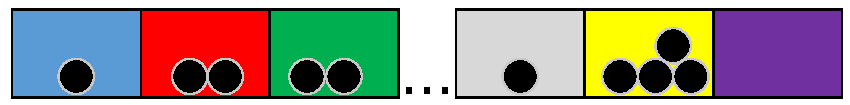
\includegraphics[width=0.5\linewidth]{mai_fig034.pdf}
    \par}

  Mezi dvěma krajními pevnými stěnami máme tedy k dispozici \(k\) pozic pro kuličky a \((n - 1)\) 
  pozic pro pohyblivé přepážky. Celkem tedy \((n + k - 1)\) pozic, na které můžeme libovolně 
  rozmísťovat \(k\) kuliček a \((n - 1)\) přepážek. Do těchto \((n + k - 1)\) pozic můžeme umístit 
  \(k\) kuliček \(C_k'(n)\) způsoby, kde
  \begin{equation}\label{MAI:eq011}
  \boxed{C_k'(n) =  
    \begin{pmatrix}
        n + k - 1 \\
        k
    \end{pmatrix} = 
    \begin{pmatrix}
        n + k - 1 \\
        n-1
    \end{pmatrix}
    }\, .
  \end{equation}
  Na zbylé pozice již musíme umístit přepážky. Nebo naopak, nejprve umístíme \((n - 1)\) přepážek a 
  potom kuličky. Výsledek je stejný, jak je vidět z předchozího vzorce. Protože jsme vytváření 
  kombinací s opakováním \(k\)-té třídy z \(n\) prvků převedli na úlohu o rozmísťování kuliček do 
  přihrádek, udává získaný vzorec právě počet takových kombinací. Aby měl vzorec smysl, musí platit 
  \(n + k - 1 \geqq k\), tedy \(n \geqq 1\).

  Komu nevyhovuje představa kuliček v přihrádkách a má raději čísla, může uvažovat následovně: Tak 
  jako je každé číslo v desítkové soustavě zapsáno pomocí cifer \(0, 1, 2, \ldots , 8, 9\), je k 
  jeho zápisu ve dvojkové soustavě potřeba pouze dvou cifer, nuly a jedničky. Představme si nyní 
  přepážku jako jedničku a kuličku jako nulu. Náš úkol zjistit počet všech možných způsobů 
  rozdělení \(k\) kuliček do \(n\) přihrádek, ohraničených \((n+1)\) přepážkami, můžeme převést na 
  ekvivalentní problém: Kolik dokážeme najít čísel, která jsou ve dvojkové soustavě zapsána právě 
  \(k\) nulami a \((n + 1)\) jedničkami, požadujeme-li, aby první i poslední cifrou byla jednička? 
  Odpověď je jednoduchá. Máme k dispozici \((n+k+1)\) pozic pro cifry. První a poslední pozice jsou 
  pevně obsazeny jedničkami, volných pozic je tedy pouze \((n + k - 1)\). Počet všech různých 
  způsobů, kterými na \(k\) z těchto pozic můžeme umístit nuly, je roven počtu kombinací \(k\)-té 
  třídy z \((n + k - 1)\) prvků. Na zbylé pozice již musíme umístit jedničky. Komplementárně, 
  budeme-li hledat počet všech možných způsobů, jak na \((n-1)\) pozic umístit jedničky, dostaneme 
  shodný výsledek, v souhlasu se vzorcem (\ref{mai:eq010}).
\normalsize
\end{example}